\documentclass[11pt, numbers=endperiod, parskip=half]{scrartcl}

\usepackage{amsmath}
\usepackage{graphicx}
\usepackage[final]{pdfpages}

\title{Assignment 4}
\subtitle{COS30023 - Languages in Software Development}
\author{Daniel Parker - 971328X}

\date{\today}

\begin{document}
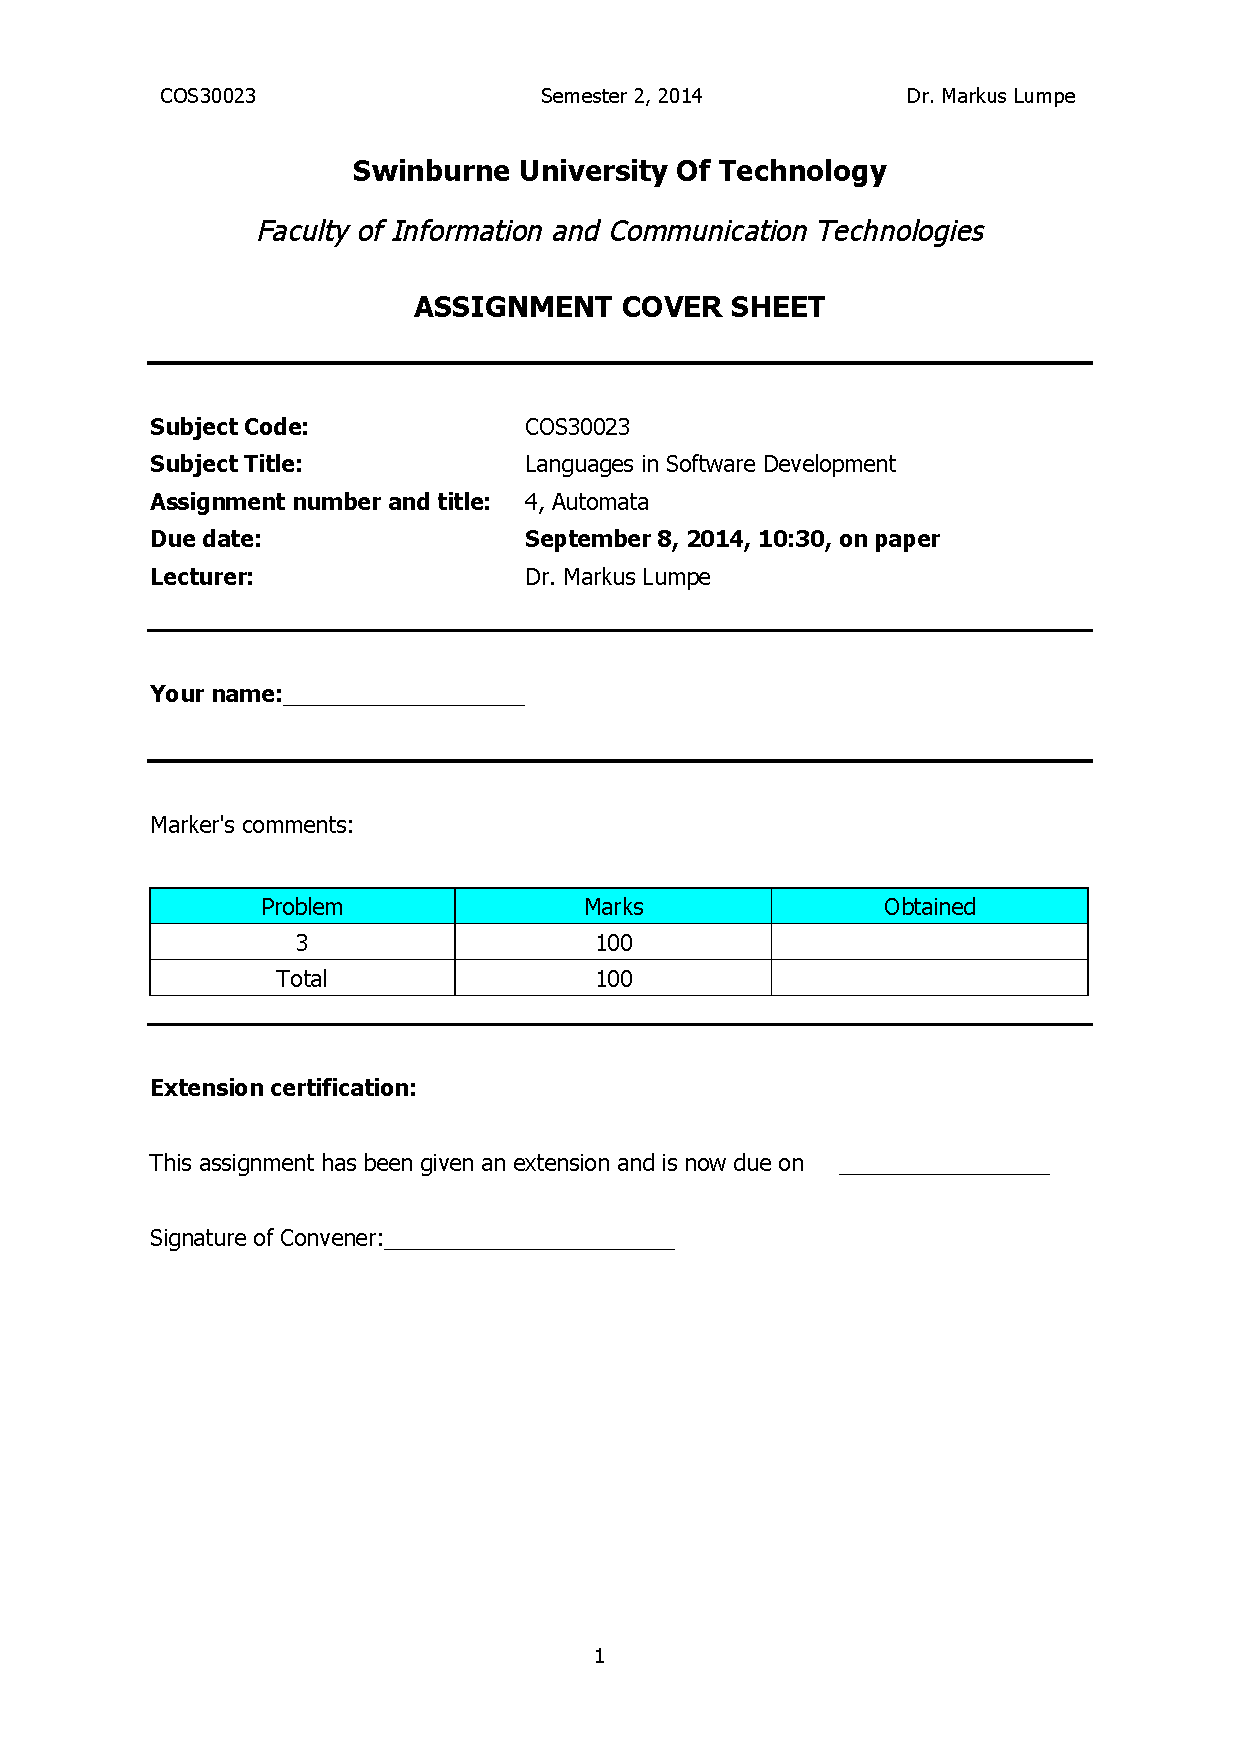
\includepdf[pages=1-1]{ProblemSet4.pdf}
\maketitle

\section{Problem 1}
\subsection{Finite Automaton}
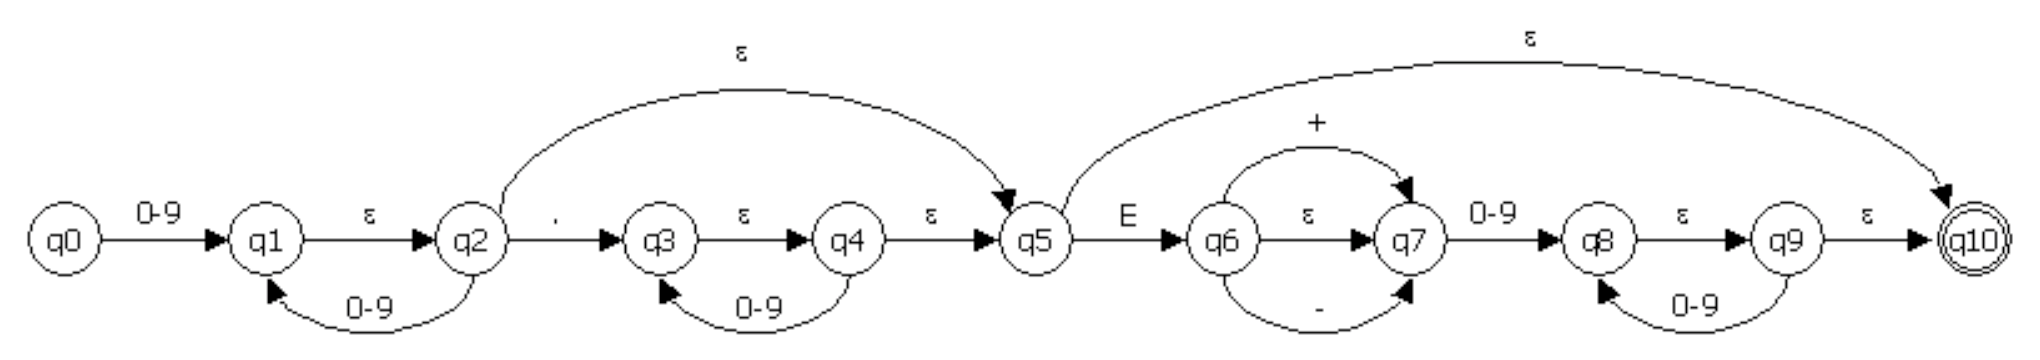
\includegraphics[scale=0.4]{automaton.png}

\subsection{Equations and Rules}
\((S_1 \cdot S_2 ) \cdot S_3 = S_1 \cdot (S_2 \cdot S_3)\)\\
\( (S_1 | S_2) \cdot T = S_1 \cdot T | S_2 \cdot T \)\\
\( T \cdot (S_1 | S_2) = T \cdot S_1 | T \cdot S_2 \)\\
\( S \cdot \epsilon = S \)\\
\( S \cdot \o = \o\)\\
\( S \cdot ( T \cdot S )^* = (S \cdot T)^* \cdot S \)

\subsubsection{Arden's Rule}
\(X = S \cdot X | T\) has solution \(S^* \cdot T\)

\subsection{Equation Set}
\(q_0 = 0-9 \oplus q_1\)\\
\(q_1 = \epsilon \oplus q_2\)\\
\(q_2 = 0-9 \oplus q_1\ |\ . \oplus q_3\ |\ \epsilon \oplus q_5 \)\\
\(q_3 = \epsilon \oplus q_4\)\\
\(q_4 = 0-9 \oplus q_3\ |\ \epsilon \oplus q_5\)\\
\(q_5 = E \oplus q_6\ |\ \epsilon \oplus q_{10}\)\\
\(q_6 = + \oplus q_7\ |\ - \oplus q_7\ |\ \epsilon \oplus q_7\)\\
\(q_7 = 0-9 \oplus q_8\)\\
\(q_8 = \epsilon \oplus q_9\)\\
\(q_9 = 0-9 \oplus q_8\ |\ \epsilon \oplus q_{10}\)\\
\(q_{10} = \epsilon\)

\subsubsection{Simplified Sets}
\(q_0 = 0-9 \oplus q_1\)\\
\(q_1 = q_2\)\\
\(q_2 = 0-9 \oplus q_1\ |\ . \oplus q_3\ |\ q_5 \)\\
\(q_3 = q_4\)\\
\(q_4 = 0-9 \oplus q_3\ |\ q_5\)\\
\(q_5 = E \oplus q_6\ |\ q_{10}\)\\
\(q_6 = (+|-|\epsilon) \oplus q_7\)\\
\(q_7 = 0-9 \oplus q_8\)\\
\(q_8 = q_9\)\\
\(q_9 = 0-9 \oplus q_8\ |\ q_{10}\)\\
\(q_{10} = \epsilon\)

\subsubsection{Substitute \(q_{10}\)}
\begin{flalign*}
q_5 &= E \oplus q_6\ |\ q_{10}\\
	&= E \oplus q_6\ |\ \epsilon
\end{flalign*}
\begin{flalign*}
q_9 &= 0-9 \oplus q_8\ |\ q_{10}\\
	&= 0-9 \oplus q_8\ |\ \epsilon\\
\end{flalign*}
\subsubsection{Substitute \(q_9\)}
\begin{flalign*}
q_8 &= 0-9 \oplus q_8\ |\ \epsilon \\
	&= (0-9)^* \oplus \epsilon\ \ \ Arden's Rule \\
	&= (0-9)^*
\end{flalign*}
\subsubsection{Substitute \(q_8\)}
\begin{flalign*}
q_7 &= 0-9 \oplus (0-9)^*
\end{flalign*}
\subsubsection{Substitute \(q_7\)}
\begin{flalign*}
q_6 &= (+|-|\epsilon) \oplus (0-9 \oplus (0-9)^*)
\end{flalign*}
\subsubsection{Substitute \(q_6\)}
\begin{flalign*}
q_5 &= E \oplus ((+|-|\epsilon)\oplus(0-9 \oplus (0-9)^*))\ |\ \epsilon
\end{flalign*}
\subsubsection{Substitute \(q_5\)}
\begin{flalign*}
q_4 &= 0-9 \oplus q_3\ |\ (E \oplus ((+|-|\epsilon)\oplus(0-9 \oplus (0-9)^*))\ |\ \epsilon)
\end{flalign*}
\begin{flalign*}
q_2 &= 0-9 \oplus q_1\ |\ . \oplus q_3\ |\ (E \oplus ((+|-|\epsilon)\oplus(0-9 \oplus (0-9)^*))\ |\ \epsilon)
\end{flalign*}
\subsubsection{Substitute \(q_4\)}
\begin{flalign*}
q_3 &= 0-9 \oplus q_3\ |\ (E \oplus ((+|-|\epsilon)\oplus(0-9 \oplus (0-9)^*))\ |\ \epsilon)\\
	&= (0-9)^* \oplus (E \oplus ((+|-|\epsilon)\oplus(0-9 \oplus (0-9)^*))\ |\ \epsilon)\ \ \ Arden's Rule
\end{flalign*}
\subsubsection{Substitute \(q_3\)}
\begin{flalign*}
q_2 &= 0-9 \oplus q_1\ \\
	&|\ . \oplus ((0-9)^* \oplus (E \oplus ((+|-|\epsilon)\oplus(0-9 \oplus (0-9)^*))\ |\ \epsilon))\ \\
	&|\ (E \oplus ((+|-|\epsilon)\oplus(0-9 \oplus (0-9)^*))\ |\ \epsilon)
\end{flalign*}
\subsubsection{Substitute \(q_2\)}
\begin{flalign*}
q_1 &= 0-9 \oplus q_1\ \\
	&|\ . \oplus ((0-9)^* \oplus (E \oplus ((+|-|\epsilon)\oplus(0-9 \oplus (0-9)^*))\ |\ \epsilon))\ \\
	&|\ (E \oplus ((+|-|\epsilon)\oplus(0-9 \oplus (0-9)^*))\ |\ \epsilon)\\
	&= (0-9)^* \oplus (. \oplus ((0-9)^* \oplus (E \oplus ((+|-|\epsilon)\oplus(0-9 \oplus (0-9)^*))\ |\ \epsilon))\ \\
	&|\ (E \oplus ((+|-|\epsilon)\oplus(0-9 \oplus (0-9)^*))\ |\ \epsilon))
\end{flalign*}
\subsubsection{Substitute\(q_1\)}
\begin{flalign*}
q_0 &= 0-9 \oplus ((0-9)^* \oplus (. \oplus ((0-9)^* \oplus (E \oplus ((+|-|\epsilon)\oplus(0-9 \oplus (0-9)^*))\ |\ \epsilon))\ \\
	&|\ (E \oplus ((+|-|\epsilon)\oplus(0-9 \oplus (0-9)^*))\ |\ \epsilon))
)
\end{flalign*}

\subsection{Regular Expression}
\[
	^\wedge [0-9]^+ \backslash.?[0-9]^* (E[+-]?[0-9]^+)?\$
\]

\subsection{Token Type}
The token defined above is an unsigned IEEE floating point number. Here are some strings that are valid in the above definition.
\begin{itemize}
	\item{\(123\)}
	\item{\(123.123\)}
	\item{\(123.123E+123\)}
	\item{\(123.123E-123\)}
	\item{\(123.123E123\)}
	\item{\(123E+123\)}
	\item{etc.}
\end{itemize}
\end{document}
